\chapter{Results}
Once all parts of this project were developed individually testing began on the physical manipulator. The main code for this project was written in python and used to call the image program to return the world coordinates of each known obstacle in the workspace. The program then calculated a path to the desired object while avoiding the others using the developed path planning code. The path was then sent over serial to the micro-controller which commanded the servos of the arm to the desired locations. 

The obstacles used to test the path planning were an orange cylinder, a blue square prism, and a green triangular prism. These objects can be seen in the figures of the image processing section.

Implementing this code made it easier to test many different object locations than it was with the modeled versions of the arm's path planning. There were a limited number of locations where obstacles could be placed that remained in the workspace of the manipulator. It was not possible to simply place an object anywhere near the manipulator and have it plan a path to it as some of the locations were not possible for it to reach.

For the obstacles within the reach of the arm's kinematics it could only pick up a few based on the two part path developed in the models. The arm would only successfully grab the obstacle when two conditions were met. The first was that the path's first approach was ended in an orientation pointing at the obstacle, rather than being at the side. The second condition was that the second part of the path, to actually do the grabbing did not cause the arm to hit the obstacle before grabbing. This problem is caused by the fact that the goal location cannot be both an obstacle and goal for the whole of path planning or the manipulator will never reach it. 

The first approach to fix this problem was to add a factor into the cost function for if the arm was pointing at the goal. The hope was that the arm would then calculated a path in which it was facing the goal and stop it from hitting the obstacle during the second part of the path planning. The issue with adding the orientation cost is that there is not enough flexibility in the manipulator workspace to get to a location and have the desired orientation. The result of adding this parameter is with a low tuning value that the arm ignores this orientation and simply takes longer to solve for the path it would have taken before, or with a higher tuning value cannot find a path within a reasonable amount of processing time. If the path calculations are not over after a minute there it does not seem to find a solution. There was no tuning value that could get the orientation parameter to improve the path planning.

The next approach was to set the end position of the first part of the path to a different location depending on the angle of the first joint. The goal is to place the arm at a position in which it is directly in front of the desired object. For example with an object directly to the front of the manipulator, at $\theta_1$ = around $0^o$ the best method was to send the manipulator to the coordinates $x_c -2 ,y_c , z_c$ where $x_c, y_c, z_c$ are the goal coordinates in inches. For $\theta_1$ values around $-90^o$ the formula was found to work best as $x_c, y_c -2, z_c$. For those in between a point two inches in from the x and y were used. For the negative angles the signs of the y were flipped. 

For the path planning algorithm to end it was required to find a distance where the arm was considered close enough to the point to stop the path planning. Since the angles were changed by a step size of three the arm would never perfectly reach the location. This was set to be within half an inch of the desired position. This means that there is some inaccuracy in the location of the end effector to the desired position. There is also some inaccuracy when calculated the position of the xyz coordinates. This accuracy is usually within a square inch of the actual location. Between these two there can be an error in the end effector location to a radius of one and a half square inches of the actual object center. Usually there is less error than this and the gripper is wide enough to grab the object for small amounts of error. 

The biggest issue of this system was the lack of feedback. The combination of error from the servos, camera location, and path planning results in a combined error of over an inch. This means that the manipulator often got close to the desired goal but not quite at the right position. The problem also arose of the error resulting in collisions with the arm and the objects. With feedback it would become much more possible to control this error resulting in a more reliable path planner. Having the gripper open as wide as possible while planning a path did help the reliability of actually grabbing the goal object, but also increased the chance of hitting other obstacles along the way.

Overall after some adjustments to the code this program was able to grab objects, while avoiding obstacles, for most locations in the workspace. With the limited workspace there is not always a path to find which can successfully grab the object without hitting it away. So while the path planner can find a smooth path to the object it was much harder to keep the arm in an orientation where it could actually pick up the object. The inaccuracy of the system was also a big contribution in the unreliable grasping.


\begin{figure}
    \centering
    \begin{subfigure}[b]{0.25\textwidth}
    	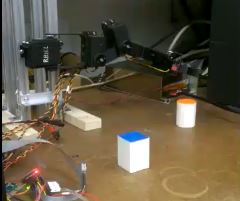
\includegraphics[width=\textwidth]{1}

   	 \end{subfigure}
   	 \quad
    \begin{subfigure}[b]{0.25\textwidth}
		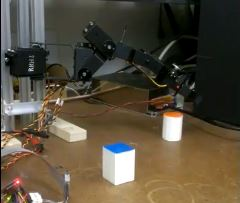
\includegraphics[width=\textwidth]{2}

    \end{subfigure}
    \quad %add desired spacing between images, e. g. ~, \quad, \qquad, \hfill etc.
    \begin{subfigure}[b]{0.25\textwidth}
        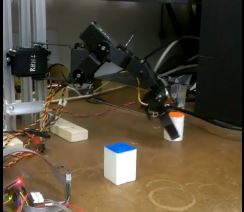
\includegraphics[width=\textwidth]{3}

    \end{subfigure}
    \quad
    \begin{subfigure}[b]{0.25\textwidth}
       	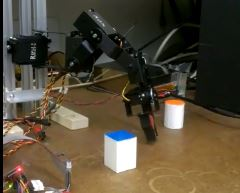
\includegraphics[width=\textwidth]{4}

   \end{subfigure}
    \quad
    \begin{subfigure}[b]{0.25\textwidth}
        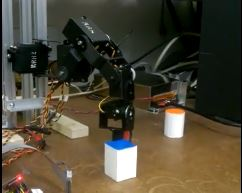
\includegraphics[width=\textwidth]{5}

    \end{subfigure}
    \quad
   	\begin{subfigure}[b]{0.25\textwidth}
        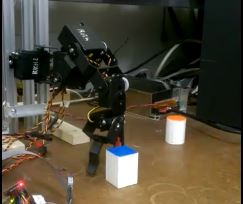
\includegraphics[width=\textwidth]{6}
    
   \end{subfigure}
   \quad
   \begin{subfigure}[b]{0.25\textwidth}
       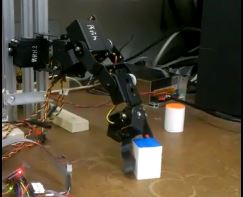
\includegraphics[width=\textwidth]{7}
        
   \end{subfigure}
   \quad
    \begin{subfigure}[b]{0.25\textwidth}
        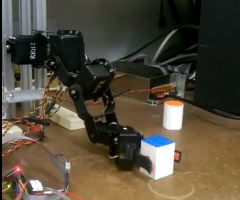
\includegraphics[width=\textwidth]{8}

    \end{subfigure}
    \quad
    \begin{subfigure}[b]{0.25\textwidth}
        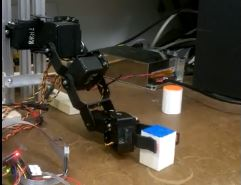
\includegraphics[width=\textwidth]{9}

    \end{subfigure}
    \quad
    \begin{subfigure}[b]{0.25\textwidth}
        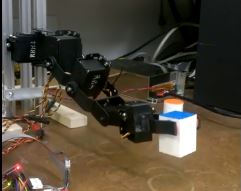
\includegraphics[width=\textwidth]{10}

    \end{subfigure}
    \quad
    \begin{subfigure}[b]{0.25\textwidth}
        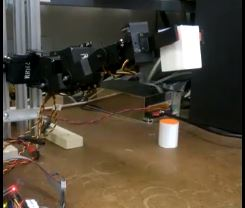
\includegraphics[width=\textwidth]{11}

    \end{subfigure}
    \quad
      %(or a blank line to force the subfigure onto a new line)
 	\caption{Manipulator moving through a planned path. }
 	\label{fig:images}
\end{figure}